 % chktex-file 13
 % chktex-file 24
 % chktex-file 44
 % chktex-file 1
 \chapter{Experimentelle Erprobung und Evaluierung}\label{ch:anomaliedetektion_test}
Im Folgenden werden die ausgewählten Algorithmen aus~\hyperref[sec:algorithmen]{Abs.~\Ref*{sec:algorithmen}} anhand realer und synthetischer
Daten getestest, evaluiert und gegenübergestellt. Ziel ist es, die Leistungsfähigkeit der verschiedenen Verfahren hinsichtlich ihrer
Erkennungsrate, Robustheit und Effizienz zu untersuchen. Dabei wird zwischen den drei Anomalietypen~–~Punkt-, Subsequenz- und
Korrelationsanomalien~–~unterschieden, um herauszufinden, welche Algorithmen sich besonders für die jeweilige Art von Abweichung eignen.

Zunächst wird die experimentelle Umgebung beschrieben, einschließlich der verwendeten Datensätze und Metriken zur Bewertung der Algorithmen.
Anschließend erfolgt die Durchführung der Experimente, wobei sowohl synthetische als auch reale Sensordaten auf Basis des SSP X1 Systems
verwendet werden. Abschließend wird eine vergleichende Analyse vorgenommen, um Stärken und Schwächen der Algorithmen herauszuarbeiten und
deren Eignung für den praktischen Einsatz in Predictive-Maintenance-Szenarien zu bewerten.

\section{Detektion von Punktanomalien}\label{sec:punktanomaliedetektion}
Zur Erprobung der Punktanomaliedetektionsalgorithmen werden drei, im Original aus den Datenaufzeichnungen der SSP X1 stammende, Ausschnitte 
der Datensätze um einige synthetische Punktanomalien erweitert. Dabei handelt es sich um die RAM und CPU Auslastung sowie die CPU Temperatur.
Die Zeitspanne, über die Daten entstanden sind, entspricht einer Dauer von genau 48 Stunden und umfasst ca.~17000 Datenpunkten, wie
in~\hyperref[fig:punktanomalien_testdata]{Abb.~\Ref*{fig:punktanomalien_testdata}} dargestellt ist.

\begin{figure}[t!]
    \centering
        \includegraphics[width=1\linewidth]{ch5_anomalieerkennung/abbildungen/punktanomalien_datensätze.pdf}
    \caption{\centering Drei Datensätze zur Gegenüberstellung und Evaluierung der beiden Algorithmen
    aus~\hyperref[tab:algorithmen]{Tab.~\Ref*{tab:algorithmen}} mit synthetisch eingefügten Anomalien, die plausible Anomaliefälle darstellen.}
~\label{fig:punktanomalien_testdata}
\end{figure}

Für die Parametrisierung der beiden Algorithmen \textbf{History Based Outlier Score} (HBOS) und \textbf{Sliding Window Z-Score} (SWZ) wurden
jeweils identische Fenstergrößen und Kontaminationsparameter übergeben. Die Kontamination gibt an, welcher relative Anteil eines Datensatzes
anomal ist und ist daher bereits eine Unsicherheit in der Analyse. Jedoch kann dies etwas eingedämmt werden, indem mehrere Durchläufe mit
variabler Kontamination durchgeführt werden. Für die Tests der drei Datensätze wurden jeweils Kontaminationswerte von 0,02 \%, 0,069 \% und
0,1 \% verwendet. Die genaue Kontamination entspricht den 0,069 \%, da 12 aus den insgesamt jeweils 17281 Datenpunkten eine Anomalie
darstellen. Bei der Analyse von Punktanomalien kann generell eine geringere Kontamination angenommen werden, da es sich nur um vereinzelte,
punktuelle Ausreißer handelt.

\begin{figure}[b!]
    \centering
        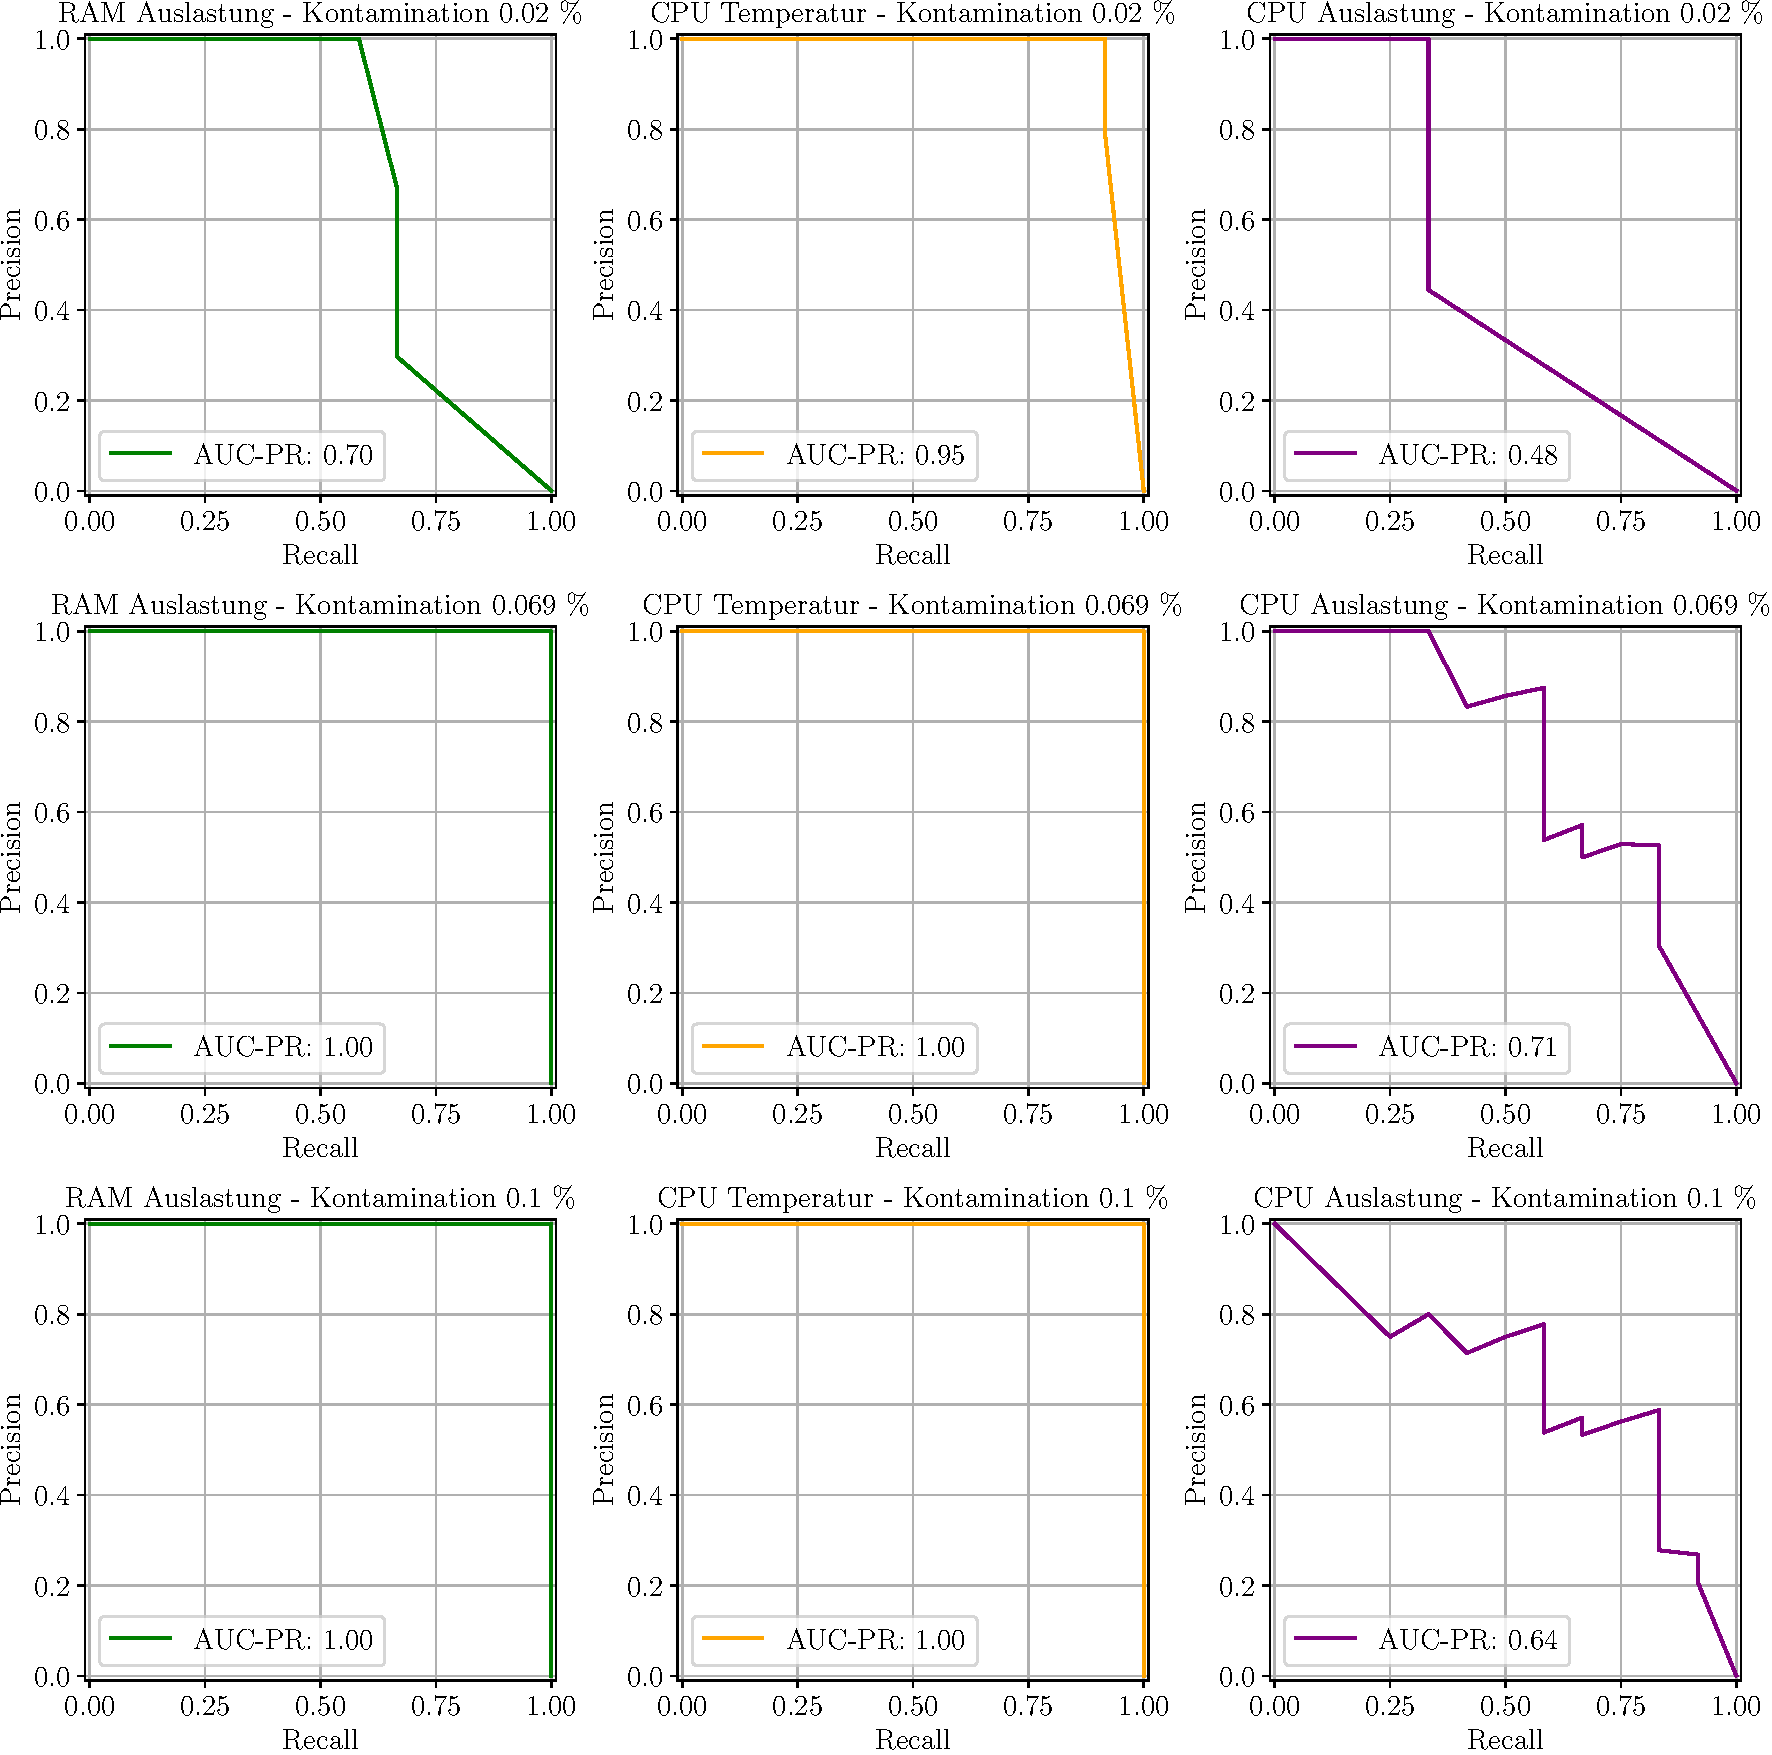
\includegraphics[width=1\linewidth]{ch5_anomalieerkennung/abbildungen/SWZ_AUC_PR.pdf}
    \caption{\centering Sliding Window Z-Score: PR-Kurven mit AUC-PR für alle drei Datensätze und die jeweiligen Kontaminationsparameter}
    \label{fig:hbos_auc_pr}
\end{figure}

\begin{figure}[t!]
    \centering
        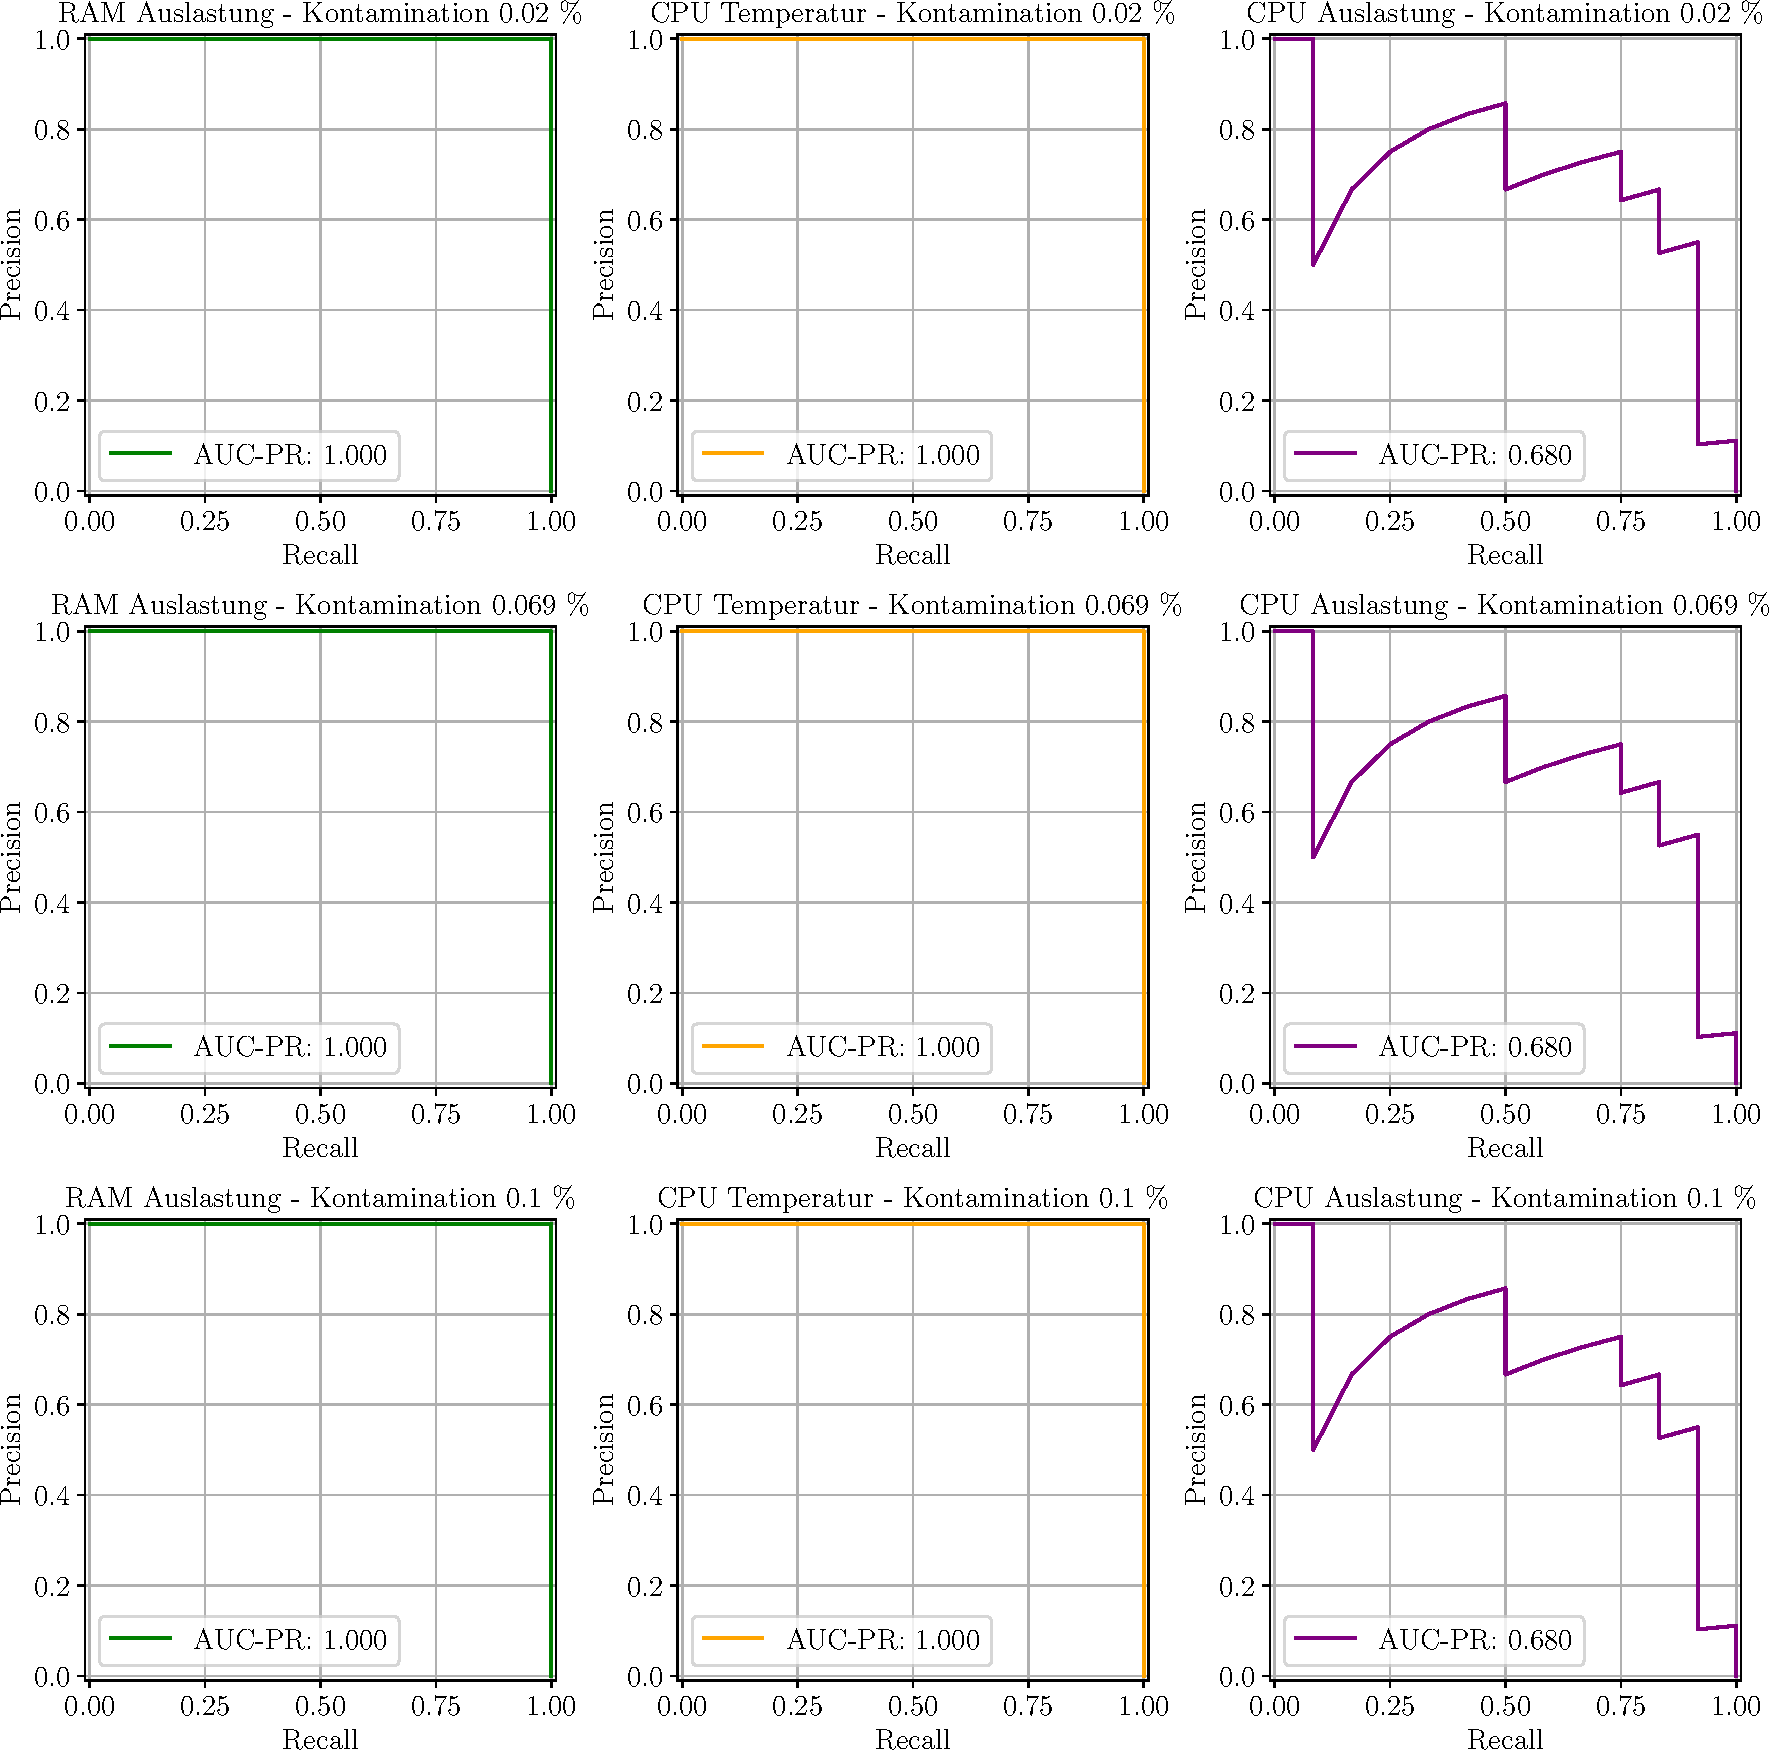
\includegraphics[width=1\linewidth]{ch5_anomalieerkennung/abbildungen/HBOS_AUC_PR.pdf}
    \caption{\centering History Based Outlier Score: PR-Kurven mit AUC-PR für alle drei Datensätze und die jeweiligen Kontaminationsparameter}
    \label{fig:swz_auc_pr}
\end{figure}

Zudem werden mehrere verschiedene Fenstergrößen benutzt, um mögliche Fehlerquellen zu eliminieren. Insgesamt werden 200 verschiedene Fenster
mit Größen zwischen 5 und 1000 Punkten eingesetzt. Für alle drei Kontaminationsparameter kann anhand der AUC-PR die Gesamtperformance des
Algorithmus über mehrere Schwellwerte abgelesen werden. Je höher die AUC-PR, desto besser ist die Performance bzw.~Präzision des Algorithmus
über mehrere Schwellen und demnach weniger abhängig von der Wahl der optimalen Schwelle, die für reale Daten ohnehin schwer zu bestimmen ist.

Auffällig ist, dass beide Algorithmen nur wenige Probleme mit den beiden Datesätzen zur RAM Auslastung sowie zur CPU Temperatur haben, während
die CPU Auslastung bei beiden schlechtere Ergebnisse aufweist. Der Grund liegt in der ungleichmäßigeren Natur der Daten, die innerhalb weniger
Datenpunkte oft Sprünge um mehrere Standardabweichungen verzeichnen. Über alle drei Kontaminationsparameter zeigt sich HBOS als der robustere
der zwei Algorithmen, während SWZ bei einer Kontamination von 0,69 \%  das beste Einzelergebnis zeigt.

Desweiteren ist zu erwähnen, dass HBOS gegenüber SWZ eine um ein Vielfaches höhere Rechendauer benötigt. Für die gezeigten Testdatensätze
betrug die Rechendauer für HBOS 150 Minuten, während SWZ die Analyse in nur 10 Sekunden abschließen konnte.

\section{Detektion von Subsequenzanomalien}
Die herausgearbeiteten Algorithmen zur Detektion von Subsequenzanomalien werden ebenfalls anhand von drei Datensätzen erprobt und evaluiert.
Ähnlich zu~\hyperref[sec:punktanomaliedetektion]{Abs.~\Ref*{sec:punktanomaliedetektion}} werden dazu die RAM Auslastung sowie die CPU Temperatur
herangezogen und um realistische Subsequenzanomalien ergänzt. Desweiteren liegt ein Datensatz zur Stromaufnahme des Blitzmoduls vor.

Als mögliches Anomalieszenario liegt für die RAM Auslastung ein plötzlicher, linearer Anstieg der Auslastung vor. Im normalen Betriebszustand
ist die Auslastung näherungsweise konstant. Im Datensatz zur CPU Temperatur wurden zwei Anomaliefälle hinzugefügt, ein sprungartiger Anstieg
sowie eine starke Schwankung im Positiven wie im Negativen. Beide Fälle entsprechen ebenfalls nicht dem Normalzustand, da die CPU Temperatur
in erster Linie von der CPU Auslastung abhängt, welche näherungsweise konstant verläuft. Außerdem korreliert die CPU Temperatur
mit der Außentemperatur, welche keinen starken Schwankungen innerhalb weniger Stunden ausgesetzt ist, wie sie im vorliegenden Anomaliefall
auftreten. Zuletzt liegen für das Blitzmodul zwei Anomaliefälle vor. Der normale zeitliche Verlauf des Blitzmoduls beschränkt sich auf einen
Ruhestrom von etwa 0,3 A sowie einen kurzen Impuls auf einen Maximalstrom von 3,5 A beim Auslösen des Blitzes. Als anomale Ereignisse liegen
zum einen ein Rippelstrom vor, dessen Problematik sich vor allem auf unerwünschtes EMV-Verhalten bezieht, und ein lang anhaltender Maximalstrom,
der entweder für einen Auslösefehler oder einen Sensordefekt hindeuten könnte. Die ursprünglichen Daten und die ergänzten Anomalien sind in
\hyperref[fig:subsequenz_datensätze]{Abb.~\Ref*{fig:subsequenz_datensätze}} aufgeführt.

Die Evaluierung der Algorithmen erfolgt ebenfalls punktbasiert mithilfe der PR-Kurve und AUC-PR, die für SWIFD
in~\hyperref[fig:SWIFD_AUC_PR]{Abb.~\Ref*{fig:SWIFD_AUC_PR}} und für LSTM-AE in einem ersten Durchlauf
in~\hyperref[fig:LSTMAE_AUC_PR_1]{Abb.~\Ref*{fig:LSTMAE_AUC_PR_1}} vorliegen. Die Untersuchung und vor allem eine aussagekräftige Evaluierung
mit GrammarViz gestaltete sich als schwierig, weshalb der Algorithmus bei der Analyse und Gegenüberstellung außen vor bleibt. LSTM-AE gehört
zur Lernklasse der Semi-Supervised Algorithmen, daher bedarf es Trainingsdaten, bevor eine Anomaliedetektion durchgeführt werden kann.

\begin{figure}[b!]
    \centering
        \includegraphics[width=1\linewidth]{ch5_anomalieerkennung/abbildungen/subsequenzanomalien_datensätze.pdf}
    \caption{\centering Drei Datensätze, anhand derer die Algorithmen zur Subsequenzanomaliedetektion getestet und evaluiert werden.}
    \label{fig:subsequenz_datensätze}
\end{figure}

\begin{figure}[t!]
    \centering
        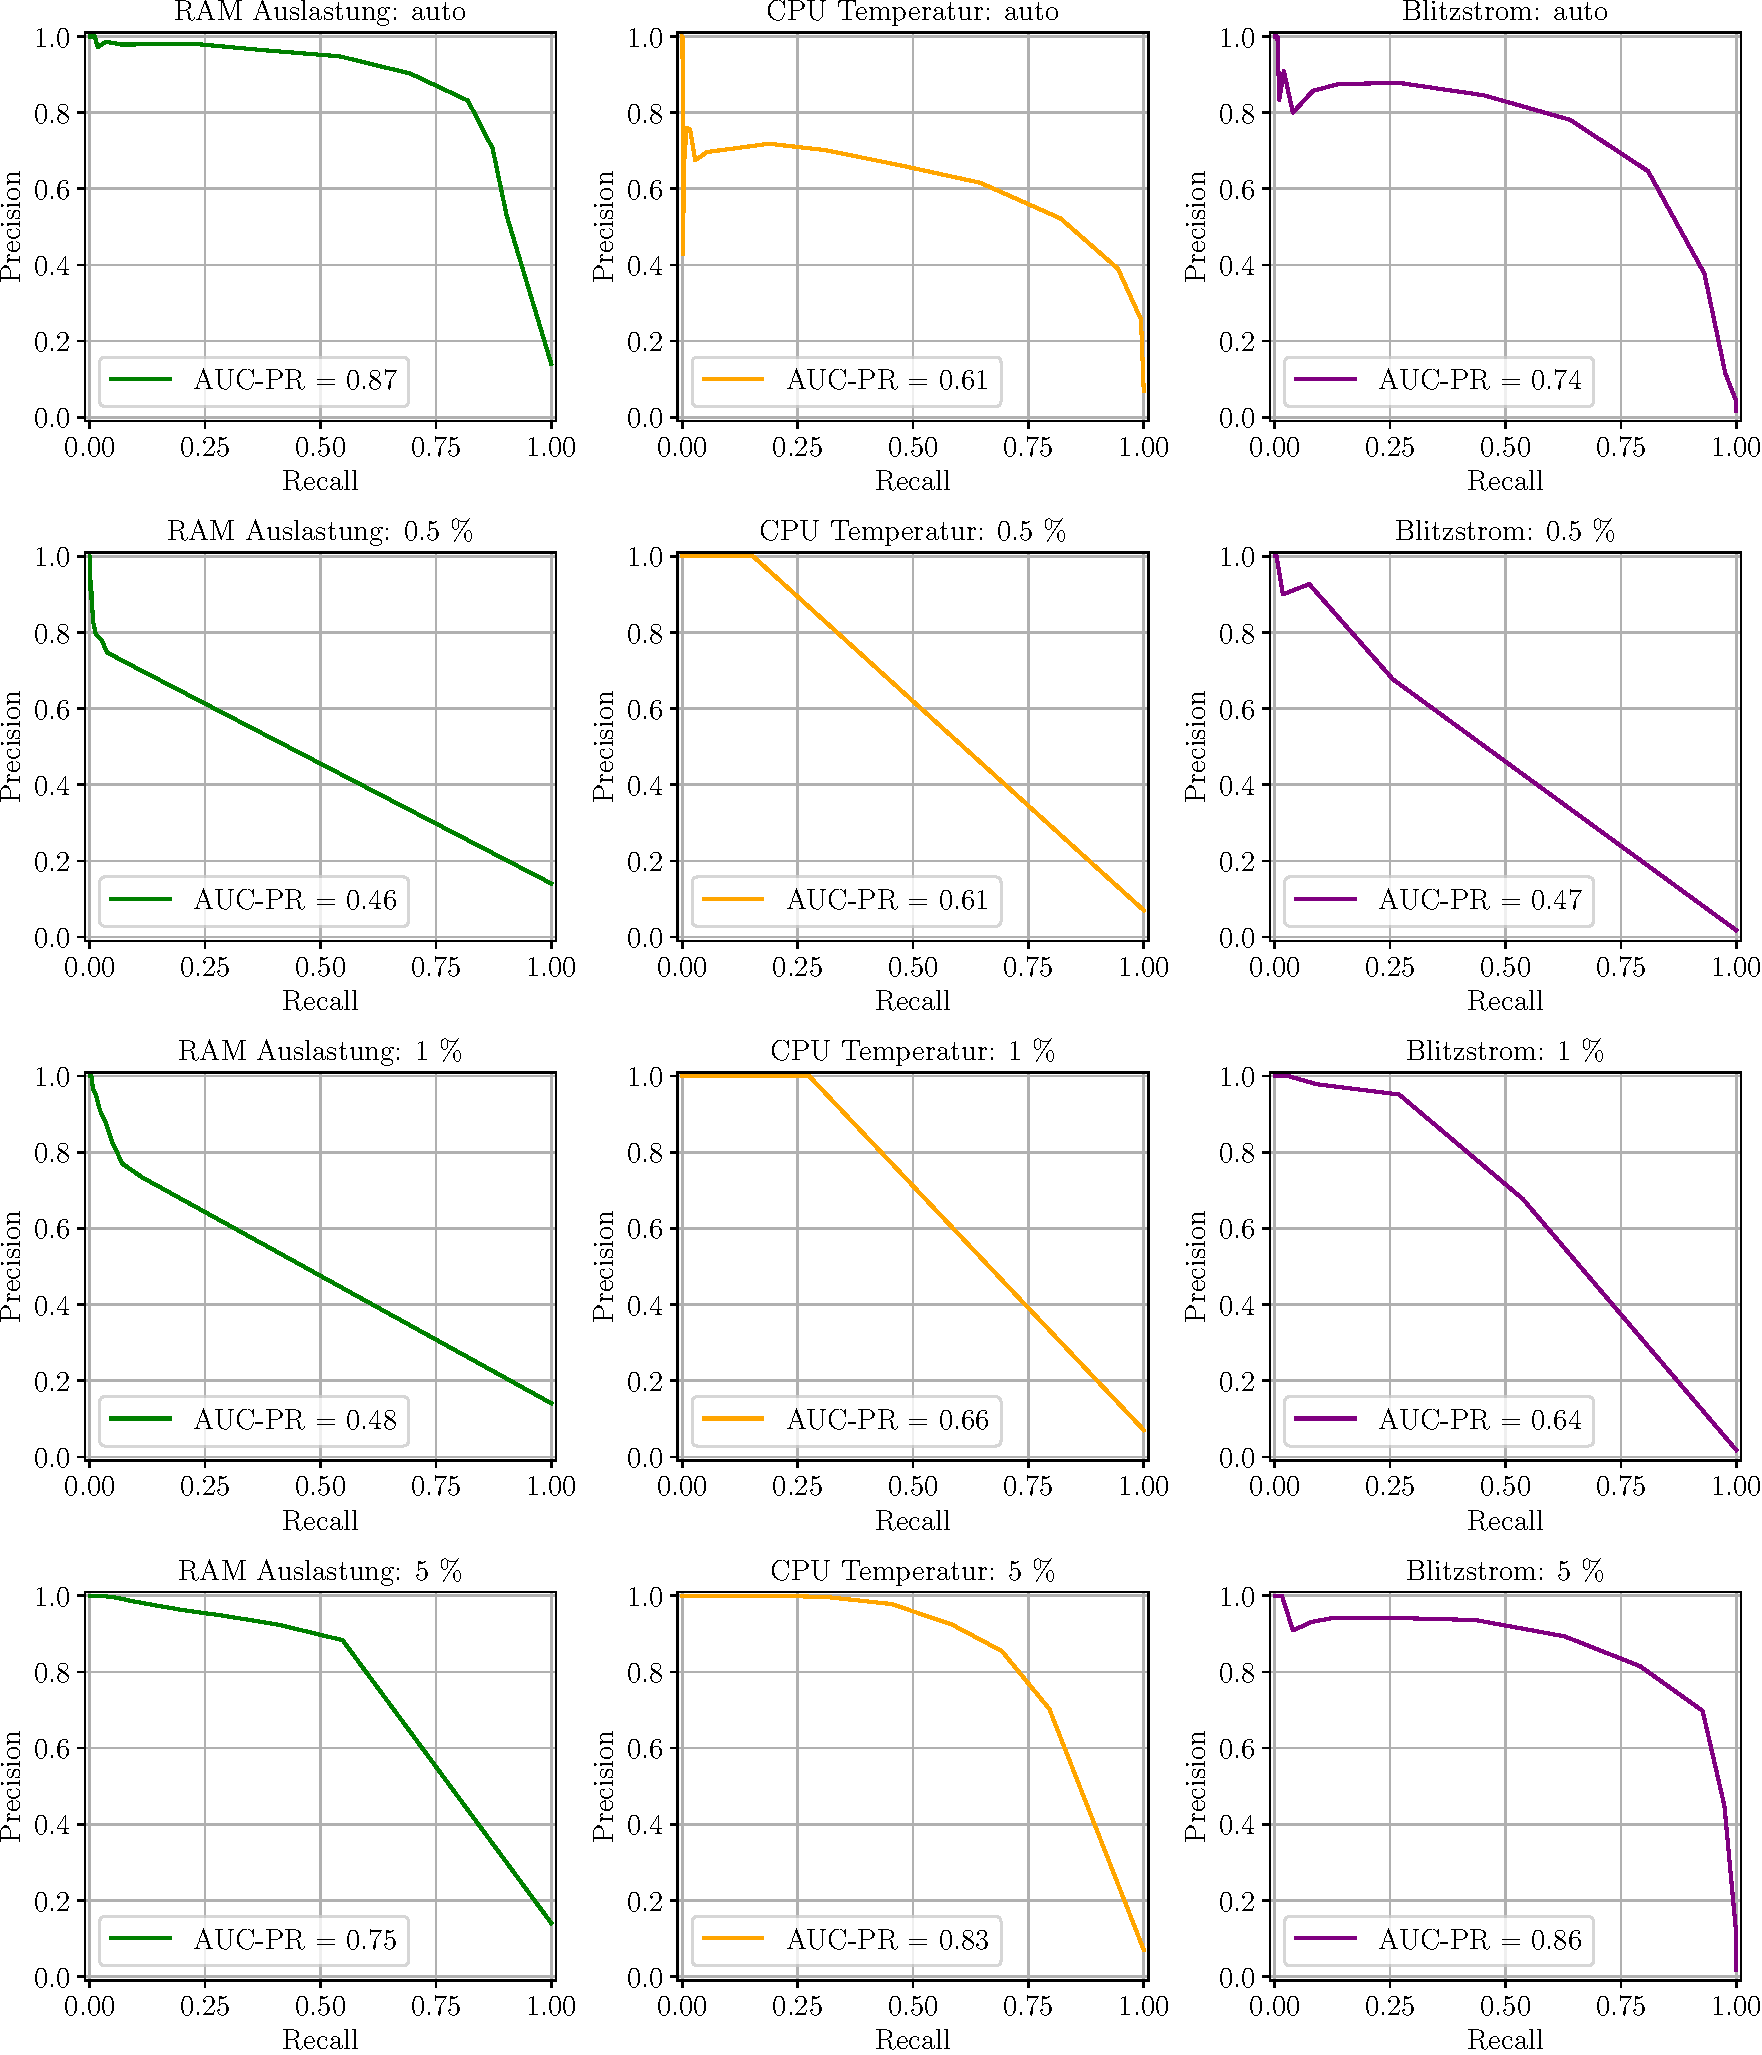
\includegraphics[width=1\linewidth]{ch5_anomalieerkennung/abbildungen/SWIFD_PR_AUC_PR.pdf}
    \caption{\centering PR-Kurven inkl. AUC-PR für alle Datensätze nach Analyse durch SWIFD mit vier Kontaminationsparametern:
    automatisch, 0,5 \%, 1 \% und 5 \%.}
    \label{fig:SWIFD_AUC_PR}
\end{figure}

Analog zu~\hyperref[sec:punktanomaliedetektion]{Abs.~\Ref*{sec:punktanomaliedetektion}} werden mehrere Fenster variabler Größe sowie mehrere
Kontaminationsparameter verwendet, um ein ganzheitliches, weniger an einzelne Parameter gebundenes, Ergebnis zu erhalten. Die Gegenüberstellung
beschränkt sich daher allein auf die PR-Kurven sowie AUC-PR, da für ein LSTM keine zusätzlichen Parameter benötigt werden, die mit denen
in SWIFD verglichen werden können. Die Performance des LSTM-AE hinsichtlich Genauigkeit und Fehlererkennungsrate bzw.~Precision und Recall
ist in aller erster Linie davon abhängig, mit welchen Hyperparametern er trainiert und initialisiert wurde~\cite{Wei2022}~\cite{Lachekhab2024}.

\begin{figure}[H]
    \centering
        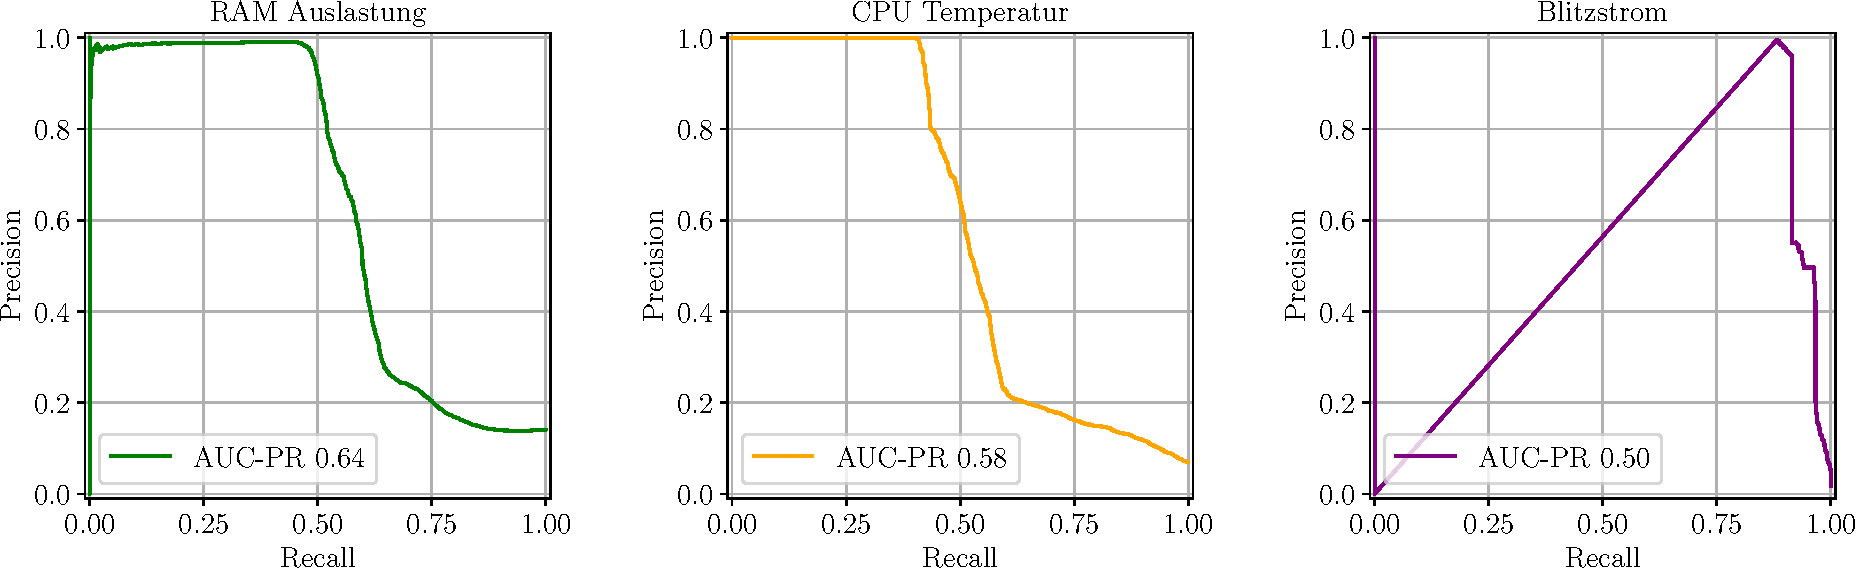
\includegraphics[width=1\linewidth]{ch5_anomalieerkennung/abbildungen/LSTMAE_PR_AUC_PR_1.pdf}
    \caption{\centering PR-Kurven und AUC-PR für das LSTM-AE Modell mit Default Parametern ohne Feintuning}
    \label{fig:LSTMAE_AUC_PR_1}
\end{figure}

\begin{figure}[b!]
    \centering
        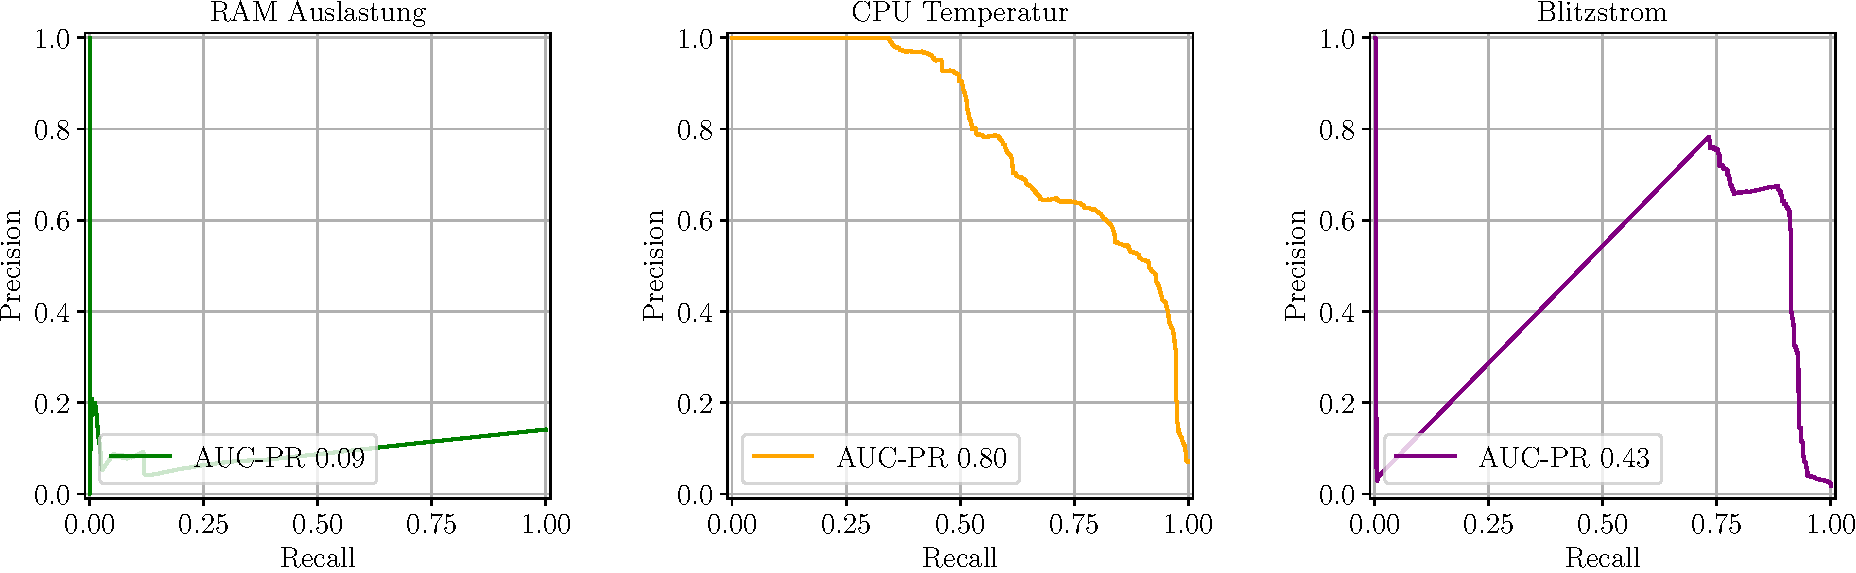
\includegraphics[width=1\linewidth]{ch5_anomalieerkennung/abbildungen/LSTMAE_PR_AUC_PR_2.pdf}
    \caption{\centering PR-Kurven und AUC-PR für das LSTM-AE Modell mit weiter angepassten Parametern wie einer erhöhten Batchgröße und mehr Epochen
    im Training.}
    \label{fig:LSTMAE_AUC_PR_2}
\end{figure}

Durch weiteres Training oder aber die Initialisierung eines neuen Modells veränderter Architektur mit Erweiterung um mehrere LSTM-Schichten
kann die Performance verbessert werden, sollte sie noch nicht zufriedenstellend sein. Allerdings bedeutet eine komplexere Architektur nicht zwangsläufig
eine genauere Vorhersage oder Detektion. Während das Training in~\hyperref[fig:LSTMAE_AUC_PR_1]{Abb.~\Ref*{fig:LSTMAE_AUC_PR_1}} mit größtenteils
voreingestellten Parametern durchgeführt wurde, so wurden danach weitere Trainings mit neuen Modellen und komplexerer Architektur durchgeführt,
die aber nicht bei allen Datensätzen zu besseren Ergebnissen führt, wie~\hyperref[fig:LSTMAE_AUC_PR_2]{Abb.~\Ref*{fig:LSTMAE_AUC_PR_2}} zeigt.

Auch die Evaluierung anhand verschiedener Metriken ist nur insoweit aussagekräftig, wie es die Qualität der Testdaten zulässt. Es liegt in der Natur
der Sache, dass reale Daten, auch wenn sie synthetisch um bestimmte Anomalien erweitert wurden, Schwankungen unterliegen, die vom menschlichen Auge
als normal eingestuft werden. Ein Algorithmus hingegen vermag ein ungewöhnliches Muster finden und es als solches markieren, und damit sein eigenes
Testergebnis verschlechtern.

Eine Ursache, dass ein Algorithmus noch keine genauen Vorhersagen treffen kann, kann auch ein noch nicht passendes Verhältnis von Trainingsdaten zu
Testdaten sein. Pauschale Annahmen, um Modelle für unterschiedliche Datensätze gleich zu trainieren, sind also offensichtlich keine zuverlässige
Herangehensweise. Hyperparameter Tuning ist ein entscheidender Schritt zur Optimierung von Machine Learning Modellen wie dem LSTM-AE, da es direkte
Auswirkungen auf die Modellleistung hat. Methoden wie Grid Search, Random Search oder Bayessche Optimierung helfen dabei, optimale Parameter zu finden,
allerdings sind sie oft rechenintensiv und erfordern große Datenmengen. Eine Herausforderung besteht darin, dass übermäßig komplexe Modelle nicht immer
zu besseren Ergebnissen führen und ein Trade-Off zwischen Overfitting und Generalisierung gefunden werden muss~\cite{Iravani2022}.

\section{Detektion von Korrelationsanomalien}

Zuletzt gilt es der Untersuchung der Algorithmen zur Korrelationsanomaliedetektion. Dazu werden drei Testdatensätze verwendet, wie sie
in~\hyperref[fig:korrelationsanomalie_datensätze]{Abb.~\Ref*{fig:korrelationsanomalie_datensätze}} dargestellt sind, mit unterschiedlichen
Szenarien, die alle eine mögliche Anomalie darlegen sollen. Die erste Anomalie beschreibt eine Verletzung der Korrelation zwischen der
CPU Last und CPU Temperatur, da die CPU Last linear steigt, während die CPU Last nicht im gleichen Maß zunimmt, sondern tendenziell abnimmt.
Der zweite Fall verletzt die Korrelation zwischen der CPU und der SOC (System On Chip~-~die Systemplatine) Temperatur, da sich diese im
Normalfall im Gleichschritt bewegen. Im vorliegenden Fall bleibt die SOC Temperatur für eine bestimmte Zeitspanne jedoch konstant, während die
CPU Temperatur ansteigt und wieder fällt. Auch der dritte abgebildete Fall stellt eine Korrelationsanomalie dar, da im selben Zeitraum die
SOC Temperatur zwar ebenfalls steigt und fällt, jedoch, im Unterschied zu allen anderen Punkten im Zeitverlauf, zeitlich versetzt.

\begin{figure}[t!]
    \centering
     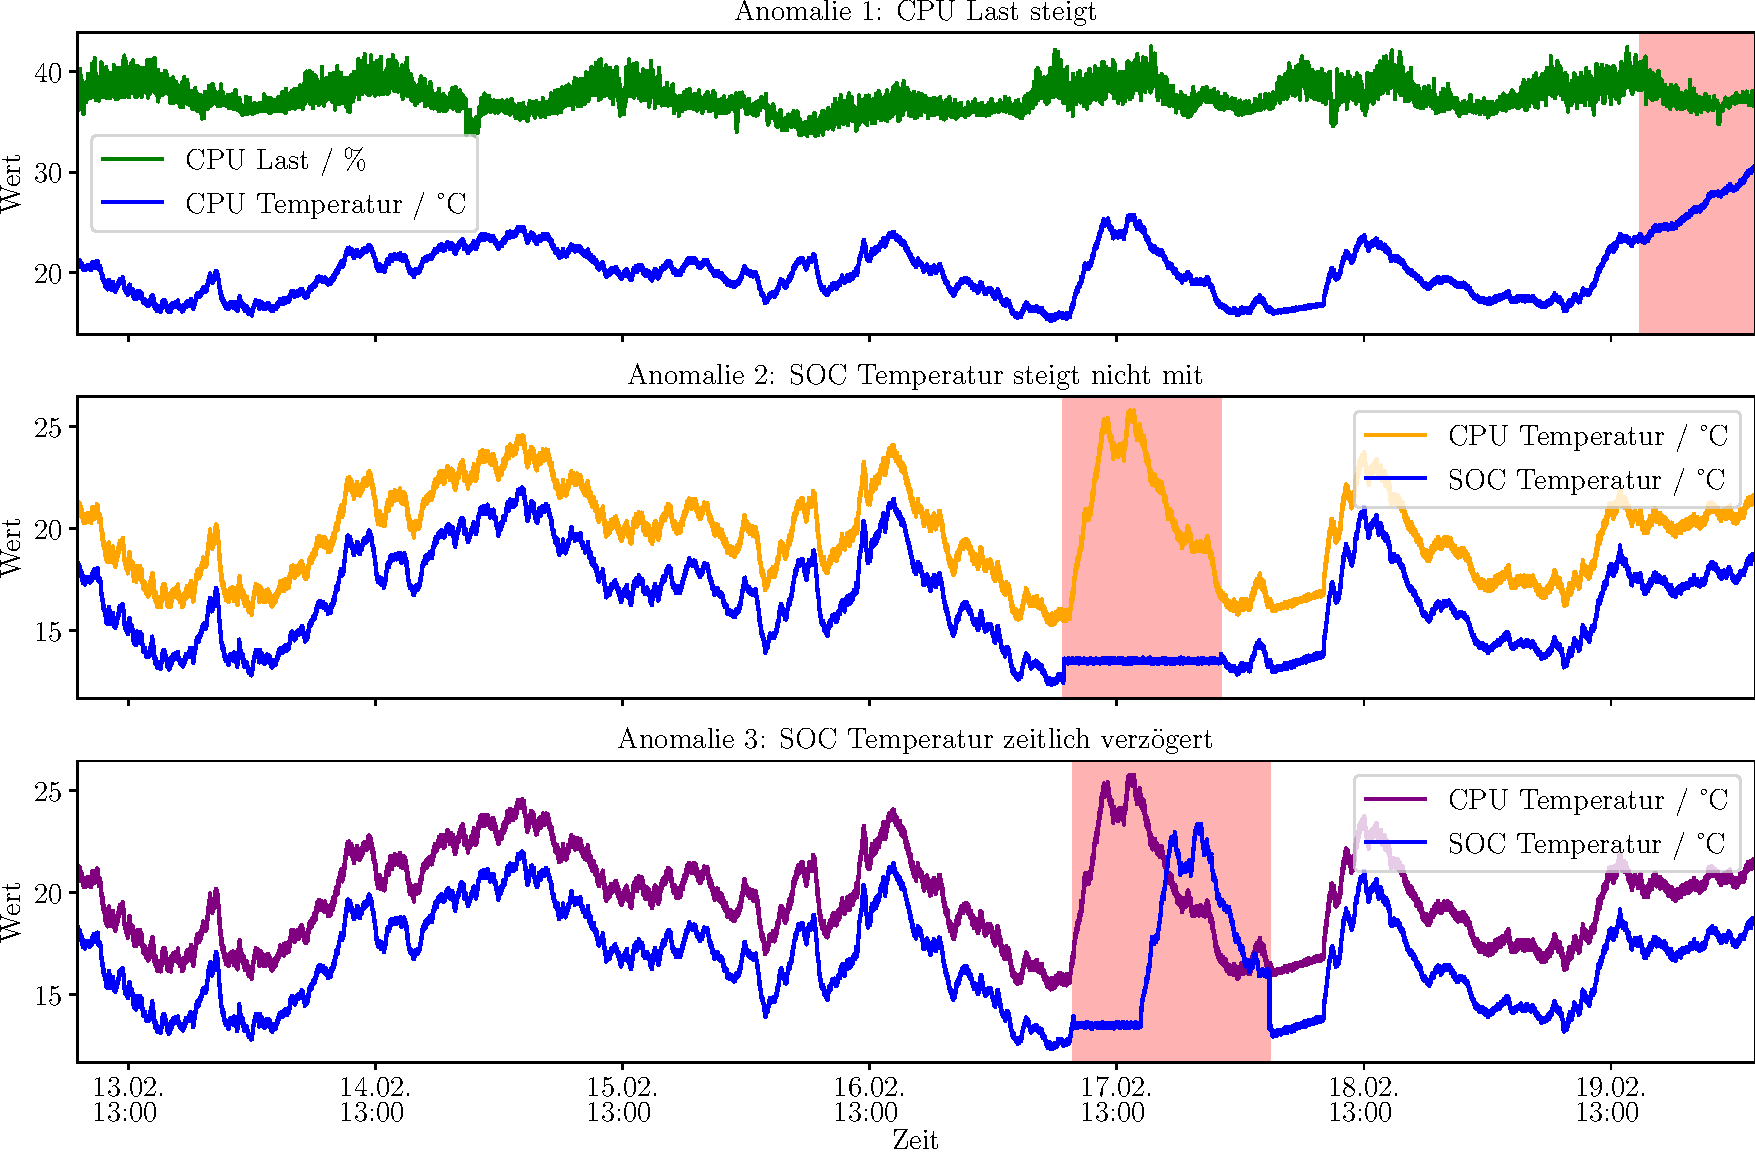
\includegraphics[width=1\linewidth]{ch5_anomalieerkennung/abbildungen/korrealtionsanomalien_daten.pdf}
    \caption{Testdatensätze mit jeweils einer Korrelationsanomalie zwischen zwei Kanälen}
    \label{fig:korrelationsanomalie_datensätze}
\end{figure}

Die untersuchten Algorithmen sind die aus~\hyperref[sec:algorithmen]{Abs.~\Ref*{sec:algorithmen}} für Korrelationsanomalien benannten MD-SWIFD und Elliptic
Envelope. Während MD-SWIFD noch mit gleitenden Fenstern arbeitet und ebenfalls, wie HBOS, SWZ und SWIFD auch mit mehreren Fenstergrößen getestet und
ausgewertet wird, benötigt Elliptic Envelope nur einen Parameter zur Angabe der erwarteten Kontmination, der für beide Algorithmen gleich übergeben wird.
Im direkten Vergleich kann Elliptic Envelope über alle Datensätze hinweg höhere AUC-PR Werte vorweisen sowie eine gänzliche Unabhängigkeit vom übergebenen
Kontaminationsparameter, was den Algorithmus zudem wesentlich handlicher im Umgang mit verschiedensten Datensätzen macht.

\begin{figure}[t!]
    \centering
        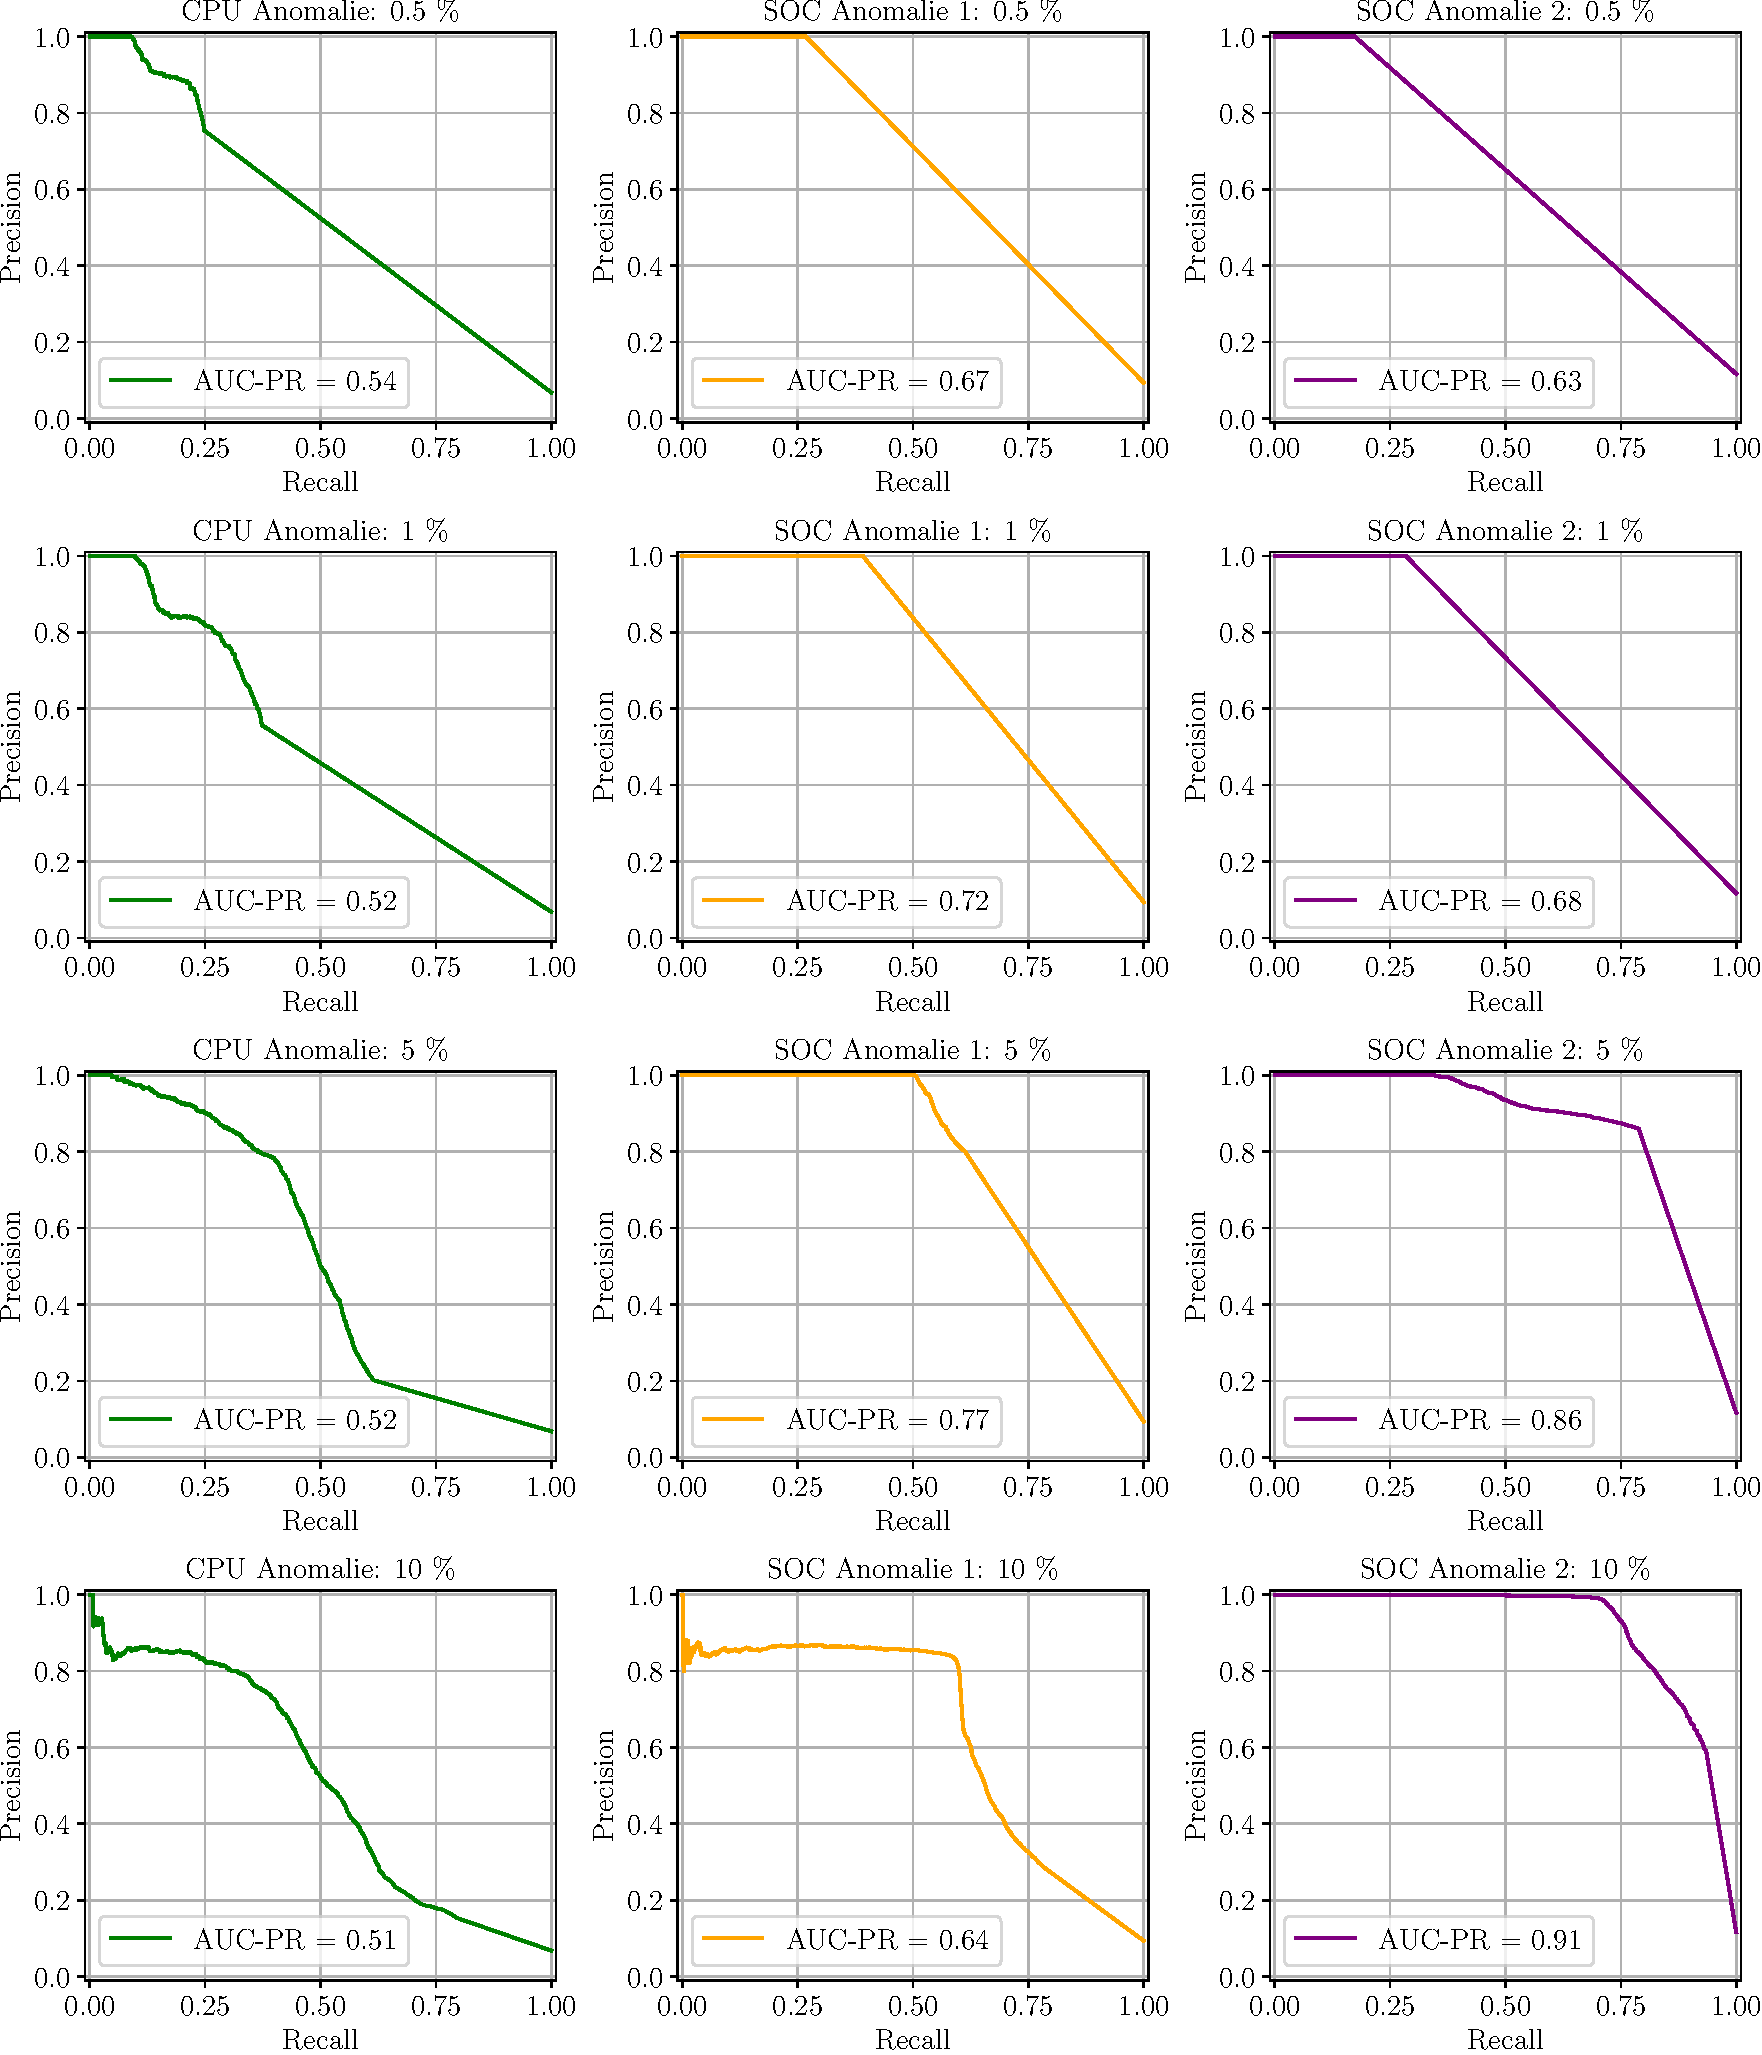
\includegraphics[width=1\linewidth]{ch5_anomalieerkennung/abbildungen/MDSWIFD_PR_AUC_PR.pdf}
    \caption{\centering PR-Kurven und AUC-PR nach der Anomaliedetektion mit MD-SWIFD. Auch hier sind die Durchläufe mit den vier
    Kontaminationsparametern 0,5 \%, 1 \%, 5 \% und 10 \% dargestellt.}
    \label{fig:MDSWIFD_AUC_PR}
\end{figure}

\begin{figure}[t!]
    \centering
        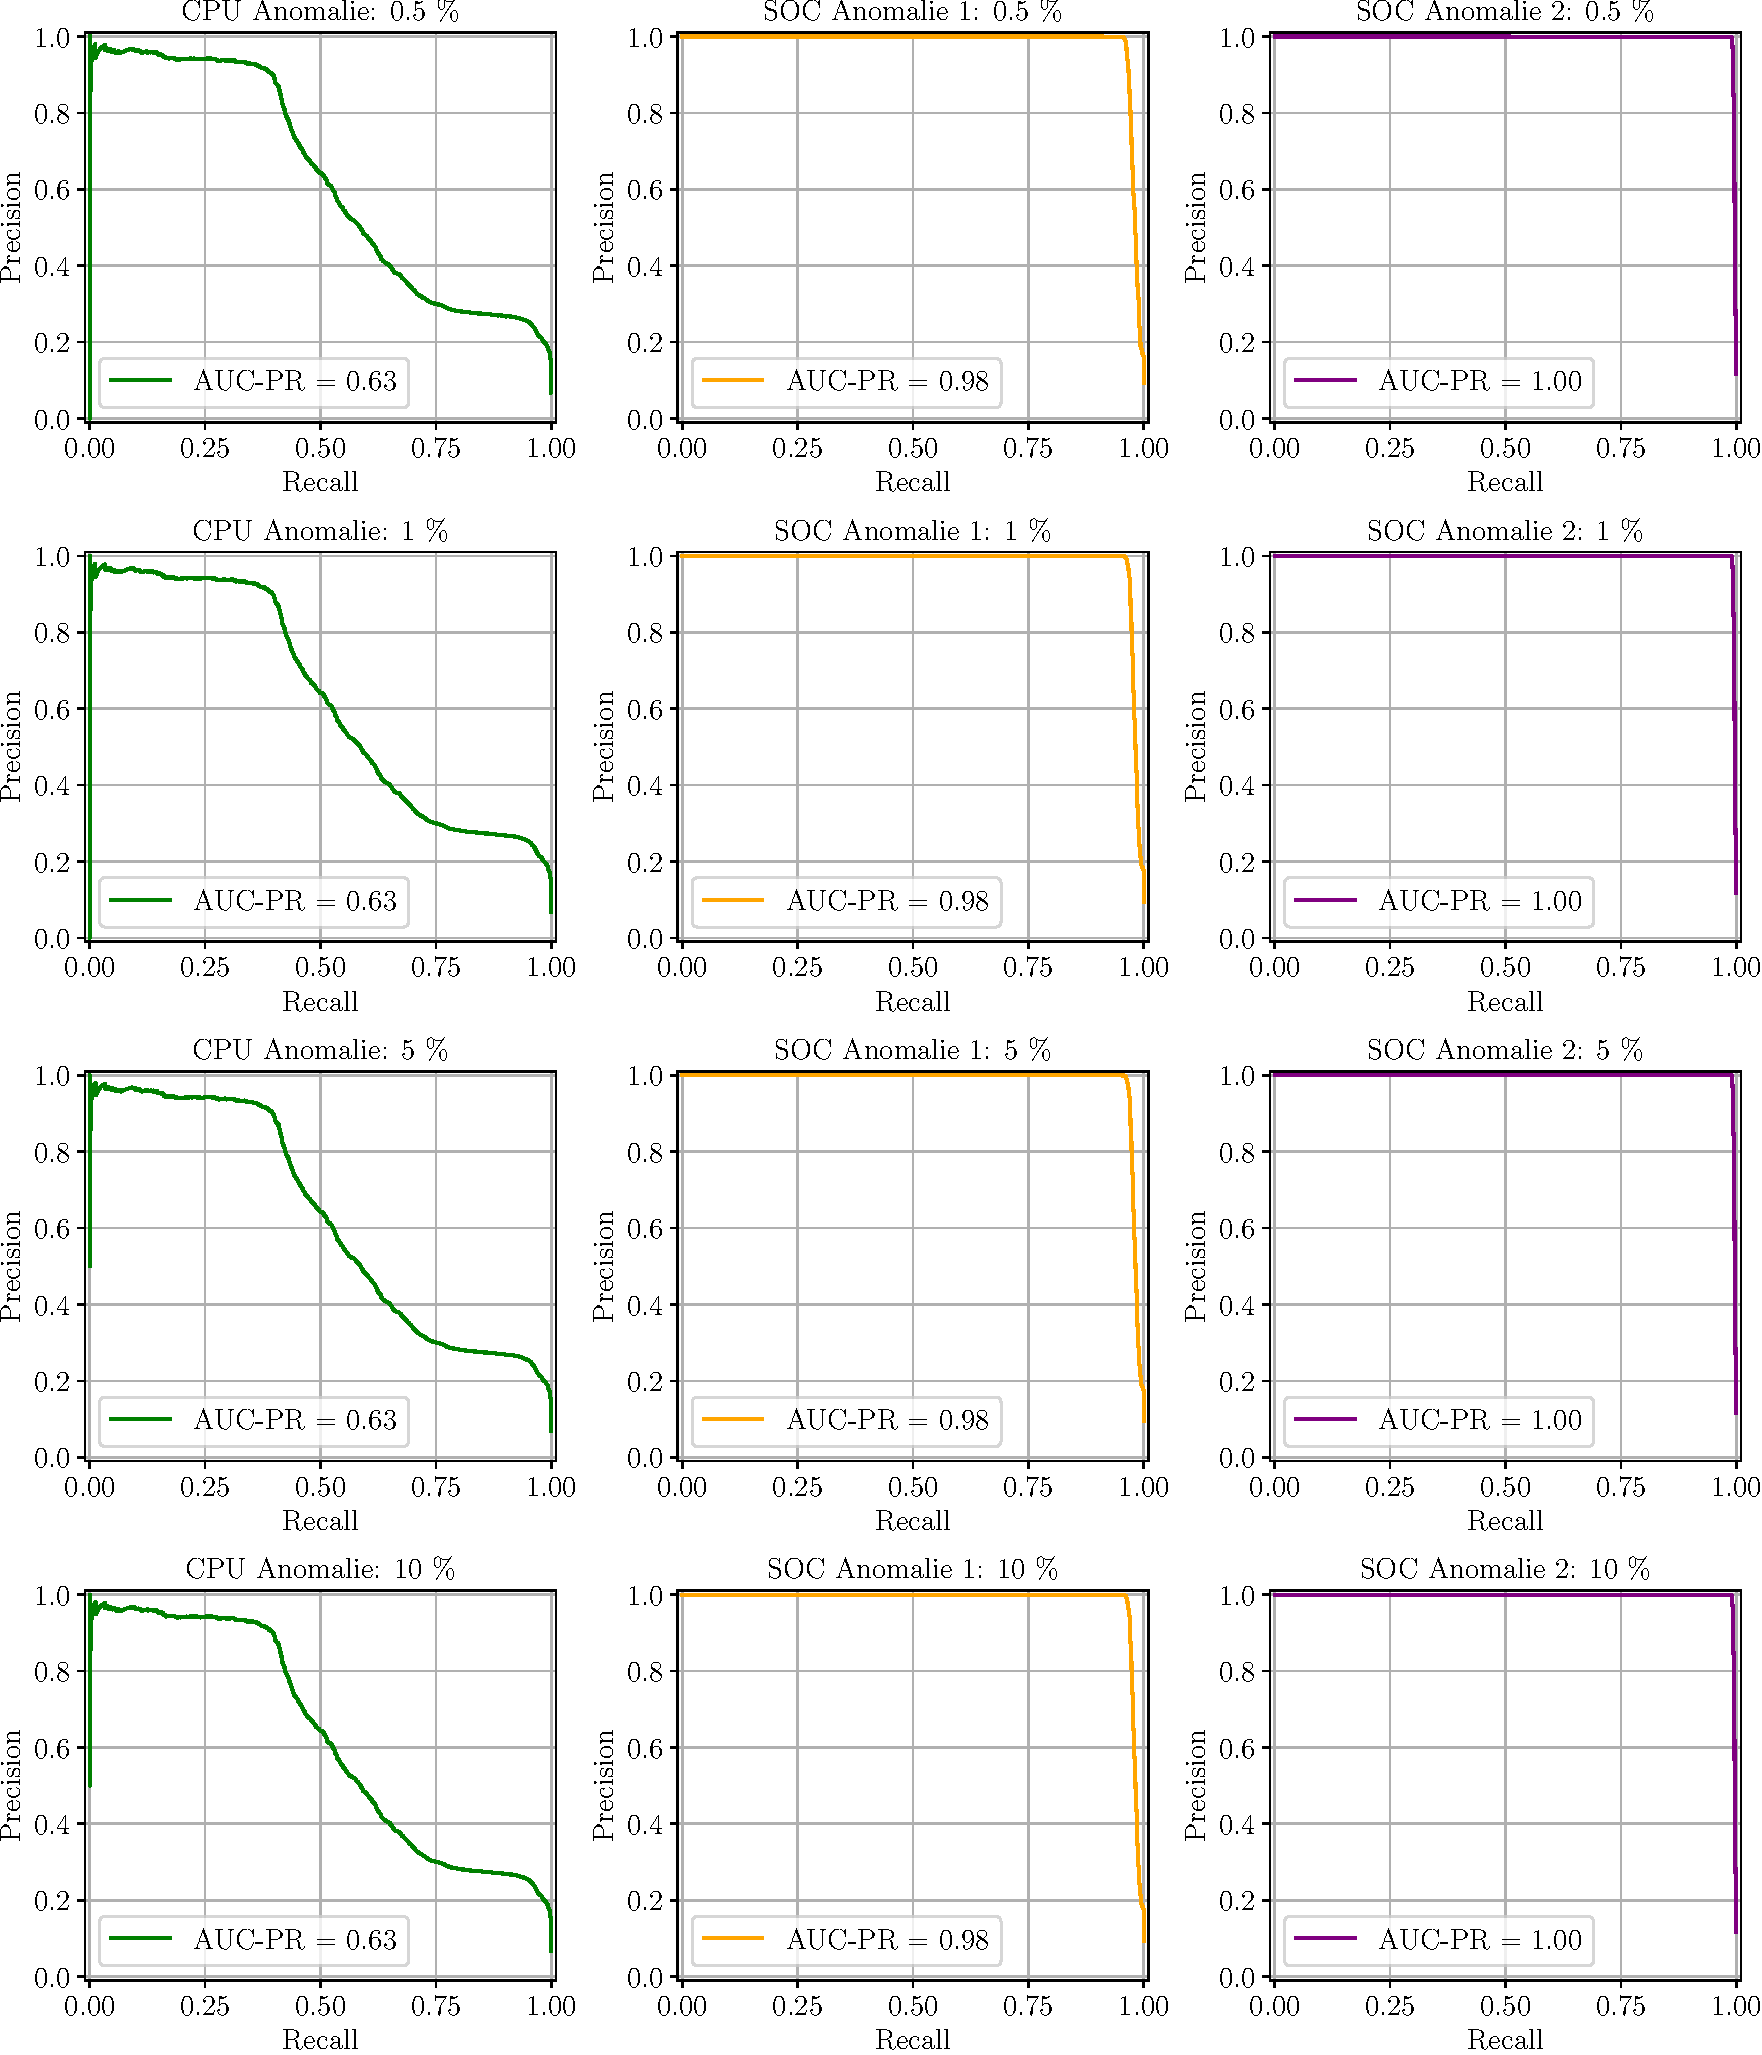
\includegraphics[width=1\linewidth]{ch5_anomalieerkennung/abbildungen/EE_PR_AUC_PR.pdf}
    \caption{\centering PR-Kurven und AUC-PR nach der Anomaliedetektion mit Elliptic Envelope. Auch hier sind die Durchläufe mit den vier
    Kontaminationsparametern 0,5 \%, 1 \%, 5 \% und 10 \% dargestellt.}
    \label{fig:EE_AUC_PR}
\end{figure}

Wie bereits bei den Algorithmen zur Subsequenzanomaliedetektion erwähnt, ist ein Testergebnis nur so aussagekräftig, wie es die Testdaten erlauben. Während
Korrelationensanomalien eindeutiger feststellbar sind als Subsequenzanomalien, wie die Ergebnisse in~\hyperref[fig:MDSWIFD_AUC_PR]{Abb.~\Ref*{fig:MDSWIFD_AUC_PR}}
und~\Ref{fig:EE_AUC_PR} zeigen, bleibt trotzdem offen, ab wann eine Korrelation wirklich
und merklich verletzt ist. Besonders Anomalie 1 wird sowohl von MD-SWIFD in~\hyperref[fig:MDSWIFD_AUC_PR]{Abb.~\Ref*{fig:MDSWIFD_AUC_PR}} als auch von Elliptic
Envelope in~\hyperref[fig:EE_AUC_PR]{Abb.~\Ref*{fig:EE_AUC_PR}} mit geringerer Genauigkeit erkannt als die anderen beiden Anomalien. Die beiden dargestellten
Variablen zur CPU Last und Temperatur sind keineswegs perfekt korreliert, aber das Verhalten der einen Größe beeinflusst zweifelsfrei das Verhalten der anderen
Größe. Aber ab wann ist eine Abweichung von diesem Verhalten groß genug, um anomal zu sein? Klar, der eingefärbte rote Bereich kann als Maßstab herangezogen werden, denn er
zeigt die Indizes, die manipuliert wurden, um die Anomalie zu erzeugen. Jedoch entspricht dieser nicht unbedingt der absoluten Wahrheit und beeinflusst trotzdem
die Ergebnisse beider Algorithmen, da AUC-PR für beide Algorithmen geringer ist als bei den anderen beiden Testdatensätzen. Die generelle Funktionalität der beiden
Algorithmen kann also anhand der beiden letzteren Anomalien, die SOC Temperatur betreffend, nachgewiesen werden, ohne dass das schlechtere Ergebnis der CPU Last Anomalie
in Fall 1 diesen Eindruck dämpfen sollte.

\clearpage
\section{Kreuzweise Überprüfung der Algorithmen}
In~\hyperref[sec:anomaliearten]{Abs.~\Ref*{sec:anomaliearten}} wurde bereits erwähnt, dass Algorithmen, die für die Detektion bestimmter Anomalien konzipiert
sind, auch in der Detektion eines breiten Spektrums verschiedener Anomalien gut abschneiden. Zur Überprüfung dieser These, die bereits mehrfach dargelegt
werden konnte~\cite[S.~30~-~31]{Wenig2024}~\cite{Schmidl2022}, sollen die selben Algorithmen aus~\hyperref[sec:algorithmen]{Abs.~\Ref*{sec:algorithmen}} deshalb
an allen anderen Datensätzen ebenfalls überprüft werden.

Trotzdem gibt es, bevor die Tests durchgeführt werden, kleine Einschränkungen bzgl.~der Eingangsdaten und damit einhergehenden möglichen Kombinationen. Die
Testdaten, die die Korrelationsanomalien enthalten, können nicht ohne Weiteres an den Algorithmen der Punkt- und Subsequenzanomalien getestet werden, da
diese nur auf univariate Zeitreihen anwendbar sind. Es können zwar multivariate Daten übergeben werden, die dann allerdings univariat verarbeitet werden, also eine
Dimension nach der anderen. Daher scheiden die zur Korrelationsanomaliedetektion generierten Daten leider aus dem Quervergleich aus. Andersherum sind die Algorithmen
zur Korrelationsanomaliedetektion sehr wohl in der Lage, univariate Daten zu untersuchen und können demnach für alle anderen Testdaten untersucht werden.

Die Detektion von Punkt- und Subsequenzanomalien wurde anhand der Algorithmen SWIFD, MD-SWIFD und Elliptic Envelope für Punktanomalien und anhand von HBOS, SWZ,
MD-SWIFD und Elliptic Envelope für Subsequenzanomalien an den Testdatensätzen aus~\hyperref[fig:punktanomalien_testdata]{Abb.~\Ref*{fig:punktanomalien_testdata}}
durchgeführt und, wie nachfolgend aufgeführt, bewertet. Dabei wurden für alle drei Algorithmen erneut mehrere verschiedene Parameter für die erwartete Kontamination
übergeben. Die AUC-PR Werte aus den jeweiligen Durchläufen werden pro Datensatz gemittelt. Die Ergebnisse der Punktanomaliedetektion liegen
in~\hyperref[tab:punktanomaliedetektion_kreuzweise]{Tab.~\Ref*{tab:punktanomaliedetektion_kreuzweise}} und~\Ref{tab:subsequenzanomaliedetektion_kreuzweise} vor.

\begin{table}[H]
    \centering
    \renewcommand{\arraystretch}{1.5} % Erhöht den Zeilenabstand für bessere Lesbarkeit
    \begin{tabular}{l|lll}
                      & \textbf{RAM Auslastung}   & \textbf{CPU Temperatur}   & \textbf{CPU Auslastung} \\
    \hline
    \textbf{SWIFD}    & \cellcolor{red!20}0,07   & \cellcolor{red!30}0,01     & \cellcolor{red!30}0,01 \\
    \textbf{MD-SWIFD} & \cellcolor{red!20}0,06   & \cellcolor{red!20}0,04     & \cellcolor{red!30}0,02 \\
    \textbf{EE}       & \cellcolor{green!40}1,0  & \cellcolor{red!5}0,25   & \cellcolor{green!25}0,78 
    \end{tabular}
    \caption{Punktanomaliedetektion durchgeführt mit den Algorithmen SWIFD, MD-SWIFD und Elliptic Envelope und Bewertung mit AUC-PR.}
    \label{tab:punktanomaliedetektion_kreuzweise}
\end{table}

\begin{table}[t!]
    \centering
    \renewcommand{\arraystretch}{1.5} % Erhöht den Zeilenabstand für bessere Lesbarkeit
    \begin{tabular}{l|lll}
                      & \textbf{RAM Auslastung}   & \textbf{CPU Temperatur}   & \textbf{Blitzstromaufnahme} \\
    \hline
    \textbf{SWZ}      & \cellcolor{red!17}0,18   & \cellcolor{red!20}0,14     & \cellcolor{red!20}0,14 \\
    \textbf{HBOS}     & \cellcolor{red!17}0,18   & \cellcolor{red!20}0,14     & \cellcolor{red!20}0,14 \\
    \textbf{MD-SWIFD} & \cellcolor{green!15}0,67 & \cellcolor{green!25}0,75   & \cellcolor{green!30}0,81 \\
    \textbf{EE}       & \cellcolor{green!30}0,85 & \cellcolor{green!10}0,55   & \cellcolor{red!12}0,2 
    \end{tabular}
    \caption{Subsequenzanomaliedetektion durchgeführt mit den Algorithmen SWZ, HBOS, MD-SWIFD und Elliptic Envelope und mit AUC-PR bewertet.}
    \label{tab:subsequenzanomaliedetektion_kreuzweise}
\end{table}

Auffällig ist das gute Abschneiden von MD-SWIFD und Elliptic Envelope, die beide zur Detektion von Korrelationensanomalien ausgewählt wurden. Ebenso auffällig
ist das unterschiedlich gute Abschneiden in den Kategorien Punkt- und Subsequenzanomalien. Die Ursache dafür findet sich im grundlegenden Funktionsprinzip der
beiden Algorithmen.

MD-SWIFD und Elliptic Envelope detektieren jeweils Anomalien auf Basis der Mahalanobis Distanz, mit dem Unterschied, dass Elliptic Envelope die Mahalanobis Distanz
Punkt für Punkt auf Anomalien untersucht und MD-SWIFD den Verlauf der Mahalanobis Distanz in Subsequenzen entspr.~der übergebenen Fenstergröße unterteilt und den
resultierenden Feature Vektor als Basis der Anomaliedetektion verwendet. Aus dem Grund schneidet Elliptic Envelope so gut für Punktanomalien ab, während MD-SWIFD
besser für die Detektion von Subsequenzanomalien geeignet ist. Weitere Auffälligkeiten sind auch durch die Natur der Daten zu begründen. Das vergleichbar schlechte
Ergebnis von Elliptic Envelope für den Datensatz der CPU Temperatur liegt vor allem am Vorhandensein vieler lokaler Anomalien, während die anderen beiden
Datensätze zur RAM und CPU Auslastung rein globale Anomalien aufweisen.

Die Mahalanobis Distanz einer Zeitreihe basiert allgemein gem.~\hyperref[eq:mahalanobis_dist]{Gl.~\Ref*{eq:mahalanobis_dist}} auf der inversen Kovarianzmatrix der
Zeitreihe. Liegt die Zeitreihe in nur einer Dimension vor, ist die Kovarianzmatrix nur noch eine Matrix der Form $1\times 1$ und somit ein Skalar, wonach sich die
Mahalanobis Distanz einer univariaten Zeitreihe vereinfachen lässt und dem Z-Score entspricht, was das Finden lokaler Anomalien als besonders schwierig gestaltet,
da sie nur im unmittelbaren Kontext anomal sind (vgl.~\hyperref[sec:punktanomalien]{Abs.~\Ref*{sec:punktanomalien}}).

Im Gegensatz dazu ermöglicht die Subsequenzanalyse der Mahalanobis Distanz das Finden ungewöhnlicher Muster, da auch die Feature Vektoren ungewöhnlicher Subsequenzen
im Vergleich zu allen anderen, normalen Subsequenzen vom Isolation Forest Algorithmus detektiert werden können.

\clearpage
\section{Diskussion der Ergebnisse}
Im Laufe des Kapitels hat sich die Unsicherheit der Testergebnisse aufgrund der Imperfektionen der Testdatensätze aufgetan. Diese lässt zwar keine absolute und
zweifelsfreie Beurteilung der getesteten Algorithmen zu, aber sie soll trotzdem nicht verhindern, dass die Performance mit Stärken und Schwächen der einzelnen
Algorithmen offen gelegt werden konnte.